\documentclass[a4paper]{article}
\usepackage{amsmath}
\usepackage{lscape}
\usepackage[margin=2.5cm]{geometry}
\usepackage{booktabs}
\usepackage{color}
\usepackage{graphicx}
\usepackage{multicol}

\title{
Flow measurement in closed conduits \\
\large{Hydraulic Engineering Experiment H6}}

\author{Mohanadas Harish Chandar \\
U067314J}
\date{September 11, 2008}

\begin{document}
\maketitle

\section{Introduction}
An experiment was conducted in a closed conduit hydraulic apparatus setup.
It consisted a venturimeter, an orifice~plate~meter, a rotameter,
a wide-angled~diffuser, and a right-angled~bend. 
The head loss across each flow meter was evaluated. 
The coefficient of discharge, $C_d$, for 
the venturimeter and the orifice~plate~meter was also determined.
The head losses and coefficients of discharge 
were then corelated with the actual discharge, $Q_A$.

\section{Objectives}
\begin{enumerate}
\item To determine the coefficient of discharge, $C_d$,
      for the
      \begin{enumerate}
      \item Venturimeter, and
      \item Orifice plate meter.
      \end{enumerate}
\item To evaluate and corelate the head losses across the 
      \begin{enumerate}
      \item Venturimeter,
      \item Orifice plate meter,
      \item Rotameter,
      \item Wide angled diffuser, and
      \item Right angled bend
      \end{enumerate}
      with the actual discharge, $Q_A$.
\end{enumerate}

\section{Procedure}
\begin{enumerate}
\item Ensure that the delivery valve is closed and start the pump.
\item Ensure that there is no air trapped in the apparatus.
\item Adjust the flow rate to the chosen level, 
      regulating only the delivery value. Ensure that the exit valve
      from the rotameter is fully open.
\item Allow flow to stabilise before taking the manometer readings.
\item Measure the time taken for 10.0\,kg of water to be collected
      in the weighing tank.
\item Repeat the procedure for eight different rates of flow.
\item At the end of the experiment close the delivery valve 
      before switching off the pump.
\end{enumerate}

\section{Experimental theory}
The measurements of discharge and head loss in this experiment 
are based on the Principle of Conservation of Energy.
The total energy of the flowing fluid is assumed 
to be constant at every cross section along the pipe.
This principle can be expressed by Bernoulli's equation,
\begin{equation}
\label{eq:bernoulli}
\frac{P_\text{X}}{\rho g}+ z_\text{X} + \frac{v^2_X}{2g}
= \frac{P_\text{Y}}{\rho g}+ z_\text{Y} + \frac{v^2_Y}{2g}, \\
\end{equation}
\begin{tabular}{rll}
where &$P$& is the pressure, and \\
      &$v$& is the mean velocity. \\
\end{tabular}

The discharge is taken to be constant at every cross-section,
giving the continuity equation,
\begin{equation}
\label{eq:continuity}
v_XA_X = v_YA_Y = Q,
\end{equation}
\begin{tabular}{rll}
where &$A$& is the area of the cross-section in consideration.
\end{tabular}

Equations for the theoretical discharge, $Q_T$,
and head loss through the various flow meters are derived from 
equations~\eqref{eq:bernoulli}~\&~\eqref{eq:continuity}.

\section{Results of the experiment}
\subsection{Sample calculations}
Below are sample calculations for the flow rate 
corresponding to a rotameter reading of 18.0\,cm.
All values listed are in the cgs system of units.

\begin{align*}
Q_A &= \frac{\text{mass of water}}{\text{density of water}} \times 
       \frac{1}{\text{time taken}} \\
    &= \frac{10000}{1} \times \frac{1}{23.08} \\
    &= 433 \\
\\
Q_T \text{ Venturi} &= A_B \sqrt{\frac{2g(h_A-h_B)}{1-(A_B/A_A)^2}} \\
                    &= 2.01 \sqrt{\frac{2\times981(35.4-14.4)}
                                      {1-2.01/5.31)^2}} \\
                    &= 441 \\
\\
C_d \text{ Venturi} &= \frac{Q_A}{Q_T} \\
                    &= \frac{433}{441} \\
                    &= 0.981 \\
\end{align*}
\begin{align*}
Q_T \text{ Orifice} &= A_F \sqrt{\frac{2g(h_E-h_F)}{1-(A_F/A_E)^2}} \\
                    &= 3.14 \sqrt{\frac{2\times981(34.2-8.0)}
                                      {1-3.14/20.43)^2}} \\
                    &= 720 \\
C_d \text{ Orifice} &= \frac{Q_A}{Q_T} \\
                    &= \frac{433}{720} \\
                    &= 0.601 \\
\end{align*}
\begin{align*}
H_V &= h_A - h_C \\
    &= 35.4 - 32.6 \\
    &= 2.8 \\
\\
H_O &= (h_E - h_F)(1 - {C_d}^2) \\
    &= (34.2 - 8.0)(1 - 0.60^2) \\
    &= 16.7 \\
\\
H_R &= h_H - h_I \\
    &= 11.6 - 0.6 \\
    &= 11.0 \\
\end{align*}
\begin{align*}
H_D &= (h_C - h_D) + \frac{{Q_A}^2}{2g}\left[\frac{1}{{A_C}^2} - 
                                             \frac{1}{{A_D}^2}\right] \\
    &= (32.6 - 33.2) + \frac{433^2}{2\times981}\left[\frac{1}{{5.31}^2} - 
                                             \frac{1}{{20.43}^2}\right] \\
    &= 2.56 \\
\\
H_B &= (h_G - h_H) + \frac{{Q_A}^2}{2g}\left[\frac{1}{{A_G}^2} - 
                                             \frac{1}{{A_H}^2}\right] \\
    &= (12.2 - 11.6) + \frac{433^2}{2\times981}\left[\frac{1}{{20.43}^2} - 
                                             \frac{1}{{5.11}^2}\right] \\
    &= -2.84 \\
\end{align*}

\begin{landscape}
\subsection{Tables}
\begin{table}[htbp]
\begin{center}
\begin{tabular}{cccccccccccc} \toprule
\multicolumn{1}{c}{Rotameter (cm)} & \multicolumn{9}{c}{Manometer Readings (mm)} & \multicolumn{2}{c}{Weighing Tank} \\ \cmidrule(r){2-10} \cmidrule(l){11-12}
\multicolumn{1}{c}{} & A & B & C & D & E & F & G & H & I & Weight (kg) & Time (s) \\ \midrule
18.0 & 354 & 144 & 326 & 332 & 342 & 80 & 122 & 116 & 6 & 10 & 23.08 \\ 
16.0 & 312 & 152 & 290 & 294 & 304 & 104 & 136 & 132 & 26 & 10 & 26.45 \\ 
14.0 & 282 & 159 & 264 & 268 & 276 & 122 & 146 & 144 & 40 & 10 & 30.21 \\ 
12.0 & 254 & 166 & 242 & 244 & 249 & 140 & 156 & 154 & 49 & 10 & 36.02 \\ 
10.0 & 232 & 170 & 222 & 223 & 228 & 153 & 164 & 162 & 56 & 10 & 44.05 \\ 
8.0 & 214 & 174 & 208 & 208 & 212 & 162 & 170 & 169 & 67 & 10 & 54.47 \\ \bottomrule
\end{tabular}
\end{center}
\caption{Measurement results}
\end{table}

\begin{table}[htbp]
\begin{center}
\begin{tabular}{ccccccccccc} \toprule
Rotameter & Q$_A$ & Q$_T$ Venturi & Q$_T$ Orifice & Venturi Loss, & Orifice Loss, & Rotameter & Wide-ang & Right-ang & Coeff. of & Coeff. of \\ 
 (cm) & (cm$^3$/s) & (cm$^3$/s) & (cm$^3$/s) & H$_V$ (cm) & H$_O$ (cm) & Loss, & Loss,  & Loss,  & discharge, & discharge, \\ 
 &  &  &  &  &  &  H$_R$ (cm) & H$_D$ (cm) & H$_B$ (cm) & C$_d$ Venturi & C$_d$ Orifice \\ \midrule
18.0 & 433 & 441 & 720 & 21.0 & 16.7 & 11.0 & 2.56 & -2.84 & 0.98 & 0.60 \\ 
16.0 & 378 & 385 & 629 & 16.0 & 12.8 & 10.6 & 2.01 & -2.22 & 0.98 & 0.60 \\ 
14.0 & 331 & 337 & 552 & 12.3 & 9.87 & 10.4 & 1.45 & -1.80 & 0.98 & 0.60 \\ 
12.0 & 278 & 285 & 465 & 8.80 & 7.01 & 10.5 & 1.10 & -1.21 & 0.97 & 0.60 \\ 
10.0 & 227 & 240 & 385 & 6.20 & 4.90 & 10.6 & 0.77 & -0.74 & 0.95 & 0.59 \\ 
8.0 & 184 & 192 & 315 & 4.00 & 3.30 & 10.2 & 0.57 & -0.52 & 0.95 & 0.58 \\ \bottomrule
\end{tabular}
\end{center}
\caption{Results from calculations}
\end{table}
\end{landscape}

\subsection{Determination of $C_d$}
\subsubsection{Venturimeter}
\begin{figure}[htbp]
\centering
% GNUPLOT: LaTeX picture with Postscript
\begingroup
  \makeatletter
  \providecommand\color[2][]{%
    \GenericError{(gnuplot) \space\space\space\@spaces}{%
      Package color not loaded in conjunction with
      terminal option `colourtext'%
    }{See the gnuplot documentation for explanation.%
    }{Either use 'blacktext' in gnuplot or load the package
      color.sty in LaTeX.}%
    \renewcommand\color[2][]{}%
  }%
  \providecommand\includegraphics[2][]{%
    \GenericError{(gnuplot) \space\space\space\@spaces}{%
      Package graphicx or graphics not loaded%
    }{See the gnuplot documentation for explanation.%
    }{The gnuplot epslatex terminal needs graphicx.sty or graphics.sty.}%
    \renewcommand\includegraphics[2][]{}%
  }%
  \providecommand\rotatebox[2]{#2}%
  \@ifundefined{ifGPcolor}{%
    \newif\ifGPcolor
    \GPcolortrue
  }{}%
  \@ifundefined{ifGPblacktext}{%
    \newif\ifGPblacktext
    \GPblacktexttrue
  }{}%
  % define a \g@addto@macro without @ in the name:
  \let\gplgaddtomacro\g@addto@macro
  % define empty templates for all commands taking text:
  \gdef\gplbacktext{}%
  \gdef\gplfronttext{}%
  \makeatother
  \ifGPblacktext
    % no textcolor at all
    \def\colorrgb#1{}%
    \def\colorgray#1{}%
  \else
    % gray or color?
    \ifGPcolor
      \def\colorrgb#1{\color[rgb]{#1}}%
      \def\colorgray#1{\color[gray]{#1}}%
      \expandafter\def\csname LTw\endcsname{\color{white}}%
      \expandafter\def\csname LTb\endcsname{\color{black}}%
      \expandafter\def\csname LTa\endcsname{\color{black}}%
      \expandafter\def\csname LT0\endcsname{\color[rgb]{1,0,0}}%
      \expandafter\def\csname LT1\endcsname{\color[rgb]{0,1,0}}%
      \expandafter\def\csname LT2\endcsname{\color[rgb]{0,0,1}}%
      \expandafter\def\csname LT3\endcsname{\color[rgb]{1,0,1}}%
      \expandafter\def\csname LT4\endcsname{\color[rgb]{0,1,1}}%
      \expandafter\def\csname LT5\endcsname{\color[rgb]{1,1,0}}%
      \expandafter\def\csname LT6\endcsname{\color[rgb]{0,0,0}}%
      \expandafter\def\csname LT7\endcsname{\color[rgb]{1,0.3,0}}%
      \expandafter\def\csname LT8\endcsname{\color[rgb]{0.5,0.5,0.5}}%
    \else
      % gray
      \def\colorrgb#1{\color{black}}%
      \def\colorgray#1{\color[gray]{#1}}%
      \expandafter\def\csname LTw\endcsname{\color{white}}%
      \expandafter\def\csname LTb\endcsname{\color{black}}%
      \expandafter\def\csname LTa\endcsname{\color{black}}%
      \expandafter\def\csname LT0\endcsname{\color{black}}%
      \expandafter\def\csname LT1\endcsname{\color{black}}%
      \expandafter\def\csname LT2\endcsname{\color{black}}%
      \expandafter\def\csname LT3\endcsname{\color{black}}%
      \expandafter\def\csname LT4\endcsname{\color{black}}%
      \expandafter\def\csname LT5\endcsname{\color{black}}%
      \expandafter\def\csname LT6\endcsname{\color{black}}%
      \expandafter\def\csname LT7\endcsname{\color{black}}%
      \expandafter\def\csname LT8\endcsname{\color{black}}%
    \fi
  \fi
  \setlength{\unitlength}{0.0500bp}%
  \begin{picture}(7200.00,5040.00)%
    \gplgaddtomacro\gplbacktext{%
      \csname LTb\endcsname%
      \put(1122,660){\makebox(0,0)[r]{\strut{}$150$}}%
      \put(1122,1346){\makebox(0,0)[r]{\strut{}$200$}}%
      \put(1122,2032){\makebox(0,0)[r]{\strut{}$250$}}%
      \put(1122,2718){\makebox(0,0)[r]{\strut{}$300$}}%
      \put(1122,3404){\makebox(0,0)[r]{\strut{}$350$}}%
      \put(1122,4090){\makebox(0,0)[r]{\strut{}$400$}}%
      \put(1122,4776){\makebox(0,0)[r]{\strut{}$450$}}%
      \put(1254,440){\makebox(0,0){\strut{}$150$}}%
      \put(2183,440){\makebox(0,0){\strut{}$200$}}%
      \put(3111,440){\makebox(0,0){\strut{}$250$}}%
      \put(4040,440){\makebox(0,0){\strut{}$300$}}%
      \put(4969,440){\makebox(0,0){\strut{}$350$}}%
      \put(5897,440){\makebox(0,0){\strut{}$400$}}%
      \put(6826,440){\makebox(0,0){\strut{}$450$}}%
      \put(220,2718){\rotatebox{90}{\makebox(0,0){\strut{}$Q_A$, (cm$^3$/s)}}}%
      \put(4040,110){\makebox(0,0){\strut{}$Q_T$, (cm$^3$/s)}}%
    }%
    \gplgaddtomacro\gplfronttext{%
      \csname LTb\endcsname%
      \put(5839,4603){\makebox(0,0)[r]{\strut{}$y=1.014x-12.76 \quad R^2=0.9996$}}%
    }%
    \gplbacktext
    \put(0,0){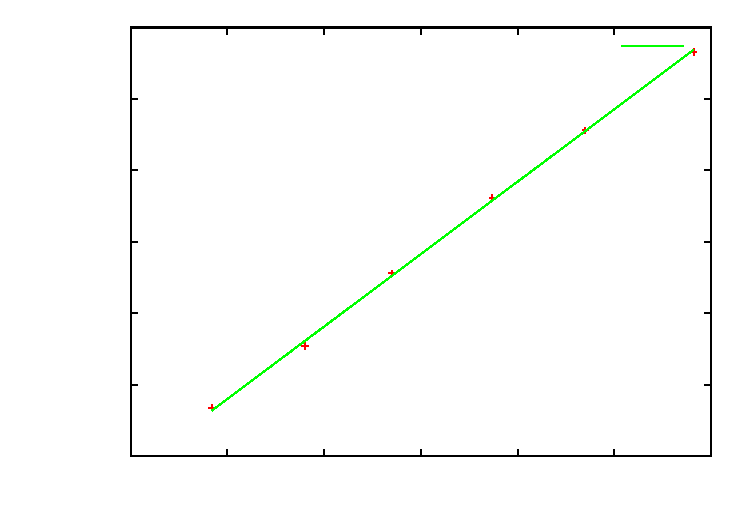
\includegraphics{qa-qt-v}}%
    \gplfronttext
  \end{picture}%
\endgroup

\caption{$Q_A$ versus $Q_T$ for the venturimeter.}
\label{fig:qa-qt-v}
\end{figure}

From figure~\ref{fig:qa-qt-v}, the following values can be determined.
\begin{align*}
n &= 6 \\
\alpha &= 0.05 \\
SS_e &= 16.50 \\
S_{xx} &= 42790 \\
t_{\alpha,n-2} &= 2.132 \\
\end{align*}

Given the above data, the 90\% confidence interval 
for the slope,~$s$ is $1.014 \pm 0.021$ and 
for the intercept,~$I$ is $-12.76 \pm 1.81$.
Removal of point 5 (240,227) gives the best improvement 
in the confidence intervals. 
The error for $s$ reduces to 0.015 and the error for $I$ reduces to 1.18.

\subsubsection{Orifice plate meter}
\begin{figure}[htbp]
\centering
% GNUPLOT: LaTeX picture with Postscript
\begingroup
  \makeatletter
  \providecommand\color[2][]{%
    \GenericError{(gnuplot) \space\space\space\@spaces}{%
      Package color not loaded in conjunction with
      terminal option `colourtext'%
    }{See the gnuplot documentation for explanation.%
    }{Either use 'blacktext' in gnuplot or load the package
      color.sty in LaTeX.}%
    \renewcommand\color[2][]{}%
  }%
  \providecommand\includegraphics[2][]{%
    \GenericError{(gnuplot) \space\space\space\@spaces}{%
      Package graphicx or graphics not loaded%
    }{See the gnuplot documentation for explanation.%
    }{The gnuplot epslatex terminal needs graphicx.sty or graphics.sty.}%
    \renewcommand\includegraphics[2][]{}%
  }%
  \providecommand\rotatebox[2]{#2}%
  \@ifundefined{ifGPcolor}{%
    \newif\ifGPcolor
    \GPcolortrue
  }{}%
  \@ifundefined{ifGPblacktext}{%
    \newif\ifGPblacktext
    \GPblacktexttrue
  }{}%
  % define a \g@addto@macro without @ in the name:
  \let\gplgaddtomacro\g@addto@macro
  % define empty templates for all commands taking text:
  \gdef\gplbacktext{}%
  \gdef\gplfronttext{}%
  \makeatother
  \ifGPblacktext
    % no textcolor at all
    \def\colorrgb#1{}%
    \def\colorgray#1{}%
  \else
    % gray or color?
    \ifGPcolor
      \def\colorrgb#1{\color[rgb]{#1}}%
      \def\colorgray#1{\color[gray]{#1}}%
      \expandafter\def\csname LTw\endcsname{\color{white}}%
      \expandafter\def\csname LTb\endcsname{\color{black}}%
      \expandafter\def\csname LTa\endcsname{\color{black}}%
      \expandafter\def\csname LT0\endcsname{\color[rgb]{1,0,0}}%
      \expandafter\def\csname LT1\endcsname{\color[rgb]{0,1,0}}%
      \expandafter\def\csname LT2\endcsname{\color[rgb]{0,0,1}}%
      \expandafter\def\csname LT3\endcsname{\color[rgb]{1,0,1}}%
      \expandafter\def\csname LT4\endcsname{\color[rgb]{0,1,1}}%
      \expandafter\def\csname LT5\endcsname{\color[rgb]{1,1,0}}%
      \expandafter\def\csname LT6\endcsname{\color[rgb]{0,0,0}}%
      \expandafter\def\csname LT7\endcsname{\color[rgb]{1,0.3,0}}%
      \expandafter\def\csname LT8\endcsname{\color[rgb]{0.5,0.5,0.5}}%
    \else
      % gray
      \def\colorrgb#1{\color{black}}%
      \def\colorgray#1{\color[gray]{#1}}%
      \expandafter\def\csname LTw\endcsname{\color{white}}%
      \expandafter\def\csname LTb\endcsname{\color{black}}%
      \expandafter\def\csname LTa\endcsname{\color{black}}%
      \expandafter\def\csname LT0\endcsname{\color{black}}%
      \expandafter\def\csname LT1\endcsname{\color{black}}%
      \expandafter\def\csname LT2\endcsname{\color{black}}%
      \expandafter\def\csname LT3\endcsname{\color{black}}%
      \expandafter\def\csname LT4\endcsname{\color{black}}%
      \expandafter\def\csname LT5\endcsname{\color{black}}%
      \expandafter\def\csname LT6\endcsname{\color{black}}%
      \expandafter\def\csname LT7\endcsname{\color{black}}%
      \expandafter\def\csname LT8\endcsname{\color{black}}%
    \fi
  \fi
  \setlength{\unitlength}{0.0500bp}%
  \begin{picture}(7200.00,5040.00)%
    \gplgaddtomacro\gplbacktext{%
      \csname LTb\endcsname%
      \put(1122,660){\makebox(0,0)[r]{\strut{}$150$}}%
      \put(1122,1346){\makebox(0,0)[r]{\strut{}$200$}}%
      \put(1122,2032){\makebox(0,0)[r]{\strut{}$250$}}%
      \put(1122,2718){\makebox(0,0)[r]{\strut{}$300$}}%
      \put(1122,3404){\makebox(0,0)[r]{\strut{}$350$}}%
      \put(1122,4090){\makebox(0,0)[r]{\strut{}$400$}}%
      \put(1122,4776){\makebox(0,0)[r]{\strut{}$450$}}%
      \put(1254,440){\makebox(0,0){\strut{}$300$}}%
      \put(1873,440){\makebox(0,0){\strut{}$350$}}%
      \put(2492,440){\makebox(0,0){\strut{}$400$}}%
      \put(3111,440){\makebox(0,0){\strut{}$450$}}%
      \put(3730,440){\makebox(0,0){\strut{}$500$}}%
      \put(4350,440){\makebox(0,0){\strut{}$550$}}%
      \put(4969,440){\makebox(0,0){\strut{}$600$}}%
      \put(5588,440){\makebox(0,0){\strut{}$650$}}%
      \put(6207,440){\makebox(0,0){\strut{}$700$}}%
      \put(6826,440){\makebox(0,0){\strut{}$750$}}%
      \put(220,2718){\rotatebox{90}{\makebox(0,0){\strut{}$Q_A$, (cm$^3$/s)}}}%
      \put(4040,110){\makebox(0,0){\strut{}$Q_T$, (cm$^3$/s)}}%
    }%
    \gplgaddtomacro\gplfronttext{%
      \csname LTb\endcsname%
      \put(5839,4603){\makebox(0,0)[r]{\strut{}$y=0.6160x-9.829 \quad R^2=0.9999$}}%
    }%
    \gplbacktext
    \put(0,0){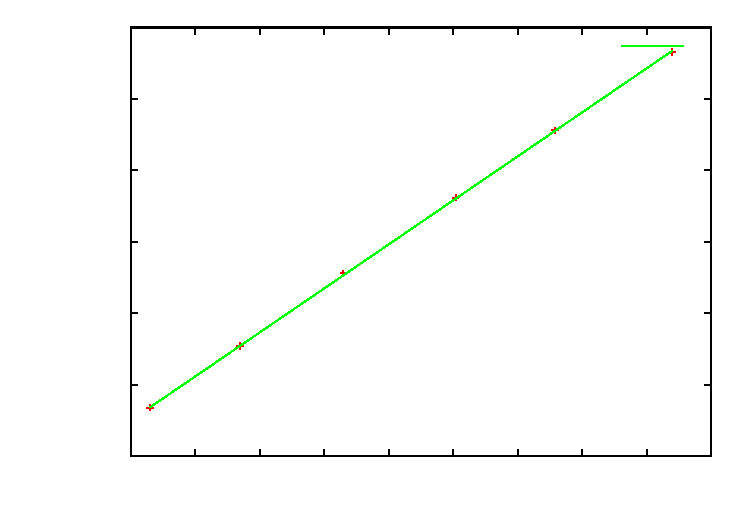
\includegraphics{qa-qt-o}}%
    \gplfronttext
  \end{picture}%
\endgroup

\caption{$Q_A$ versus $Q_T$ for the orifice plate meter.}
\label{fig:qa-qt-o}
\end{figure}
From figure~\ref{fig:qa-qt-o}, the following values can be determined.
\begin{align*}
n &= 6 \\
\alpha &= 0.05 \\
SS_e &= 2.872 \\
S_{xx} &= 11600 \\
t_{\alpha,n-2} &= 2.132 \\
\end{align*}

Given the above data, the 90\% confidence interval 
for the slope,~$s$ is $0.6160 \pm 0.0053$ and 
for the intercept,~$I$ is $-9.829 \pm 0.747$.
Removal of point 4 (465,278) gives the best improvement 
in the confidence intervals. 
The error for $s$ reduces to 0.0038 and the error for $I$ reduces to 0.532.

\subsubsection{Comments on $C_d$ values}
\begin{figure}[htbp]
\centering
% GNUPLOT: LaTeX picture with Postscript
\begingroup
  \makeatletter
  \providecommand\color[2][]{%
    \GenericError{(gnuplot) \space\space\space\@spaces}{%
      Package color not loaded in conjunction with
      terminal option `colourtext'%
    }{See the gnuplot documentation for explanation.%
    }{Either use 'blacktext' in gnuplot or load the package
      color.sty in LaTeX.}%
    \renewcommand\color[2][]{}%
  }%
  \providecommand\includegraphics[2][]{%
    \GenericError{(gnuplot) \space\space\space\@spaces}{%
      Package graphicx or graphics not loaded%
    }{See the gnuplot documentation for explanation.%
    }{The gnuplot epslatex terminal needs graphicx.sty or graphics.sty.}%
    \renewcommand\includegraphics[2][]{}%
  }%
  \providecommand\rotatebox[2]{#2}%
  \@ifundefined{ifGPcolor}{%
    \newif\ifGPcolor
    \GPcolortrue
  }{}%
  \@ifundefined{ifGPblacktext}{%
    \newif\ifGPblacktext
    \GPblacktexttrue
  }{}%
  % define a \g@addto@macro without @ in the name:
  \let\gplgaddtomacro\g@addto@macro
  % define empty templates for all commands taking text:
  \gdef\gplbacktext{}%
  \gdef\gplfronttext{}%
  \makeatother
  \ifGPblacktext
    % no textcolor at all
    \def\colorrgb#1{}%
    \def\colorgray#1{}%
  \else
    % gray or color?
    \ifGPcolor
      \def\colorrgb#1{\color[rgb]{#1}}%
      \def\colorgray#1{\color[gray]{#1}}%
      \expandafter\def\csname LTw\endcsname{\color{white}}%
      \expandafter\def\csname LTb\endcsname{\color{black}}%
      \expandafter\def\csname LTa\endcsname{\color{black}}%
      \expandafter\def\csname LT0\endcsname{\color[rgb]{1,0,0}}%
      \expandafter\def\csname LT1\endcsname{\color[rgb]{0,1,0}}%
      \expandafter\def\csname LT2\endcsname{\color[rgb]{0,0,1}}%
      \expandafter\def\csname LT3\endcsname{\color[rgb]{1,0,1}}%
      \expandafter\def\csname LT4\endcsname{\color[rgb]{0,1,1}}%
      \expandafter\def\csname LT5\endcsname{\color[rgb]{1,1,0}}%
      \expandafter\def\csname LT6\endcsname{\color[rgb]{0,0,0}}%
      \expandafter\def\csname LT7\endcsname{\color[rgb]{1,0.3,0}}%
      \expandafter\def\csname LT8\endcsname{\color[rgb]{0.5,0.5,0.5}}%
    \else
      % gray
      \def\colorrgb#1{\color{black}}%
      \def\colorgray#1{\color[gray]{#1}}%
      \expandafter\def\csname LTw\endcsname{\color{white}}%
      \expandafter\def\csname LTb\endcsname{\color{black}}%
      \expandafter\def\csname LTa\endcsname{\color{black}}%
      \expandafter\def\csname LT0\endcsname{\color{black}}%
      \expandafter\def\csname LT1\endcsname{\color{black}}%
      \expandafter\def\csname LT2\endcsname{\color{black}}%
      \expandafter\def\csname LT3\endcsname{\color{black}}%
      \expandafter\def\csname LT4\endcsname{\color{black}}%
      \expandafter\def\csname LT5\endcsname{\color{black}}%
      \expandafter\def\csname LT6\endcsname{\color{black}}%
      \expandafter\def\csname LT7\endcsname{\color{black}}%
      \expandafter\def\csname LT8\endcsname{\color{black}}%
    \fi
  \fi
  \setlength{\unitlength}{0.0500bp}%
  \begin{picture}(7200.00,5040.00)%
    \gplgaddtomacro\gplbacktext{%
      \csname LTb\endcsname%
      \put(1122,660){\makebox(0,0)[r]{\strut{}$0.5$}}%
      \put(1122,1346){\makebox(0,0)[r]{\strut{}$0.6$}}%
      \put(1122,2032){\makebox(0,0)[r]{\strut{}$0.7$}}%
      \put(1122,2718){\makebox(0,0)[r]{\strut{}$0.8$}}%
      \put(1122,3404){\makebox(0,0)[r]{\strut{}$0.9$}}%
      \put(1122,4090){\makebox(0,0)[r]{\strut{}$1$}}%
      \put(1122,4776){\makebox(0,0)[r]{\strut{}$1.1$}}%
      \put(1254,440){\makebox(0,0){\strut{}$150$}}%
      \put(2183,440){\makebox(0,0){\strut{}$200$}}%
      \put(3111,440){\makebox(0,0){\strut{}$250$}}%
      \put(4040,440){\makebox(0,0){\strut{}$300$}}%
      \put(4969,440){\makebox(0,0){\strut{}$350$}}%
      \put(5897,440){\makebox(0,0){\strut{}$400$}}%
      \put(6826,440){\makebox(0,0){\strut{}$450$}}%
      \put(220,2718){\rotatebox{90}{\makebox(0,0){\strut{}$C_d$, (cm$^3$/s)}}}%
      \put(4040,110){\makebox(0,0){\strut{}$Q_A$, (cm$^3$/s)}}%
    }%
    \gplgaddtomacro\gplfronttext{%
      \csname LTb\endcsname%
      \put(5839,4603){\makebox(0,0)[r]{\strut{}Venturimeter}}%
      \csname LTb\endcsname%
      \put(5839,4383){\makebox(0,0)[r]{\strut{}Orifice plate meter}}%
    }%
    \gplbacktext
    \put(0,0){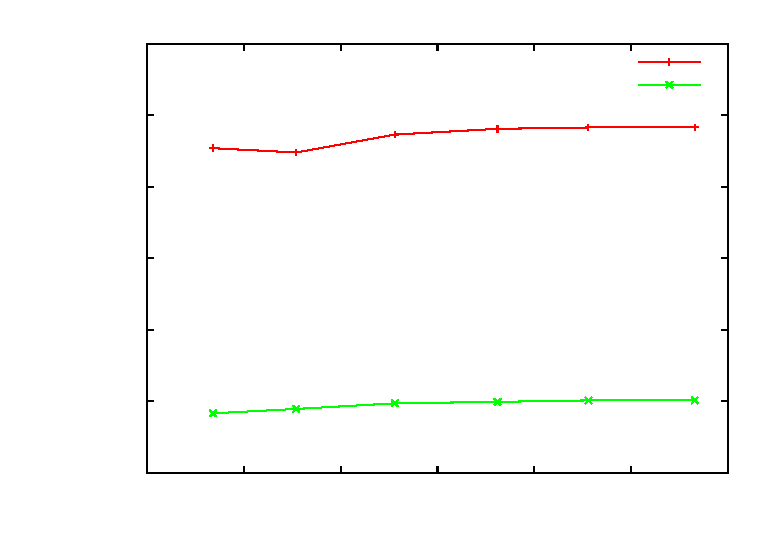
\includegraphics{cd-qa}}%
    \gplfronttext
  \end{picture}%
\endgroup

\caption{$C_d$ versus $Q_A$ for the venturimeter and the orifice plate meter.}
\label{fig:cd-qa}
\end{figure}
The differing values of $C_d$ at different rates of flow, $Q_A$, 
are shown in figure~\ref{fig:cd-qa}. The values of $C_d$ for both
the venturimeter and the orifice plate meter seem to stabilise
at higher rates of flow. Thus, the correct value of $C_d$ 
should be 0.983 for the venturimeter and 
0.601 for the orifice plate meter. This is attributed to the fact that
the flow is more stable at higer values of $Q_A$. 

\subsection{Corelation between head losses and $Q_A$}
\begin{figure}[htbp]
\centering
% GNUPLOT: LaTeX picture with Postscript
\begingroup
  \makeatletter
  \providecommand\color[2][]{%
    \GenericError{(gnuplot) \space\space\space\@spaces}{%
      Package color not loaded in conjunction with
      terminal option `colourtext'%
    }{See the gnuplot documentation for explanation.%
    }{Either use 'blacktext' in gnuplot or load the package
      color.sty in LaTeX.}%
    \renewcommand\color[2][]{}%
  }%
  \providecommand\includegraphics[2][]{%
    \GenericError{(gnuplot) \space\space\space\@spaces}{%
      Package graphicx or graphics not loaded%
    }{See the gnuplot documentation for explanation.%
    }{The gnuplot epslatex terminal needs graphicx.sty or graphics.sty.}%
    \renewcommand\includegraphics[2][]{}%
  }%
  \providecommand\rotatebox[2]{#2}%
  \@ifundefined{ifGPcolor}{%
    \newif\ifGPcolor
    \GPcolortrue
  }{}%
  \@ifundefined{ifGPblacktext}{%
    \newif\ifGPblacktext
    \GPblacktexttrue
  }{}%
  % define a \g@addto@macro without @ in the name:
  \let\gplgaddtomacro\g@addto@macro
  % define empty templates for all commands taking text:
  \gdef\gplbacktext{}%
  \gdef\gplfronttext{}%
  \makeatother
  \ifGPblacktext
    % no textcolor at all
    \def\colorrgb#1{}%
    \def\colorgray#1{}%
  \else
    % gray or color?
    \ifGPcolor
      \def\colorrgb#1{\color[rgb]{#1}}%
      \def\colorgray#1{\color[gray]{#1}}%
      \expandafter\def\csname LTw\endcsname{\color{white}}%
      \expandafter\def\csname LTb\endcsname{\color{black}}%
      \expandafter\def\csname LTa\endcsname{\color{black}}%
      \expandafter\def\csname LT0\endcsname{\color[rgb]{1,0,0}}%
      \expandafter\def\csname LT1\endcsname{\color[rgb]{0,1,0}}%
      \expandafter\def\csname LT2\endcsname{\color[rgb]{0,0,1}}%
      \expandafter\def\csname LT3\endcsname{\color[rgb]{1,0,1}}%
      \expandafter\def\csname LT4\endcsname{\color[rgb]{0,1,1}}%
      \expandafter\def\csname LT5\endcsname{\color[rgb]{1,1,0}}%
      \expandafter\def\csname LT6\endcsname{\color[rgb]{0,0,0}}%
      \expandafter\def\csname LT7\endcsname{\color[rgb]{1,0.3,0}}%
      \expandafter\def\csname LT8\endcsname{\color[rgb]{0.5,0.5,0.5}}%
    \else
      % gray
      \def\colorrgb#1{\color{black}}%
      \def\colorgray#1{\color[gray]{#1}}%
      \expandafter\def\csname LTw\endcsname{\color{white}}%
      \expandafter\def\csname LTb\endcsname{\color{black}}%
      \expandafter\def\csname LTa\endcsname{\color{black}}%
      \expandafter\def\csname LT0\endcsname{\color{black}}%
      \expandafter\def\csname LT1\endcsname{\color{black}}%
      \expandafter\def\csname LT2\endcsname{\color{black}}%
      \expandafter\def\csname LT3\endcsname{\color{black}}%
      \expandafter\def\csname LT4\endcsname{\color{black}}%
      \expandafter\def\csname LT5\endcsname{\color{black}}%
      \expandafter\def\csname LT6\endcsname{\color{black}}%
      \expandafter\def\csname LT7\endcsname{\color{black}}%
      \expandafter\def\csname LT8\endcsname{\color{black}}%
    \fi
  \fi
  \setlength{\unitlength}{0.0500bp}%
  \begin{picture}(7200.00,5040.00)%
    \gplgaddtomacro\gplbacktext{%
      \csname LTb\endcsname%
      \put(990,660){\makebox(0,0)[r]{\strut{}$-5$}}%
      \put(990,1248){\makebox(0,0)[r]{\strut{}$0$}}%
      \put(990,1836){\makebox(0,0)[r]{\strut{}$5$}}%
      \put(990,2424){\makebox(0,0)[r]{\strut{}$10$}}%
      \put(990,3012){\makebox(0,0)[r]{\strut{}$15$}}%
      \put(990,3600){\makebox(0,0)[r]{\strut{}$20$}}%
      \put(990,4188){\makebox(0,0)[r]{\strut{}$25$}}%
      \put(990,4776){\makebox(0,0)[r]{\strut{}$30$}}%
      \put(1122,440){\makebox(0,0){\strut{}$150$}}%
      \put(2073,440){\makebox(0,0){\strut{}$200$}}%
      \put(3023,440){\makebox(0,0){\strut{}$250$}}%
      \put(3974,440){\makebox(0,0){\strut{}$300$}}%
      \put(4925,440){\makebox(0,0){\strut{}$350$}}%
      \put(5875,440){\makebox(0,0){\strut{}$400$}}%
      \put(6826,440){\makebox(0,0){\strut{}$450$}}%
      \put(220,2718){\rotatebox{90}{\makebox(0,0){\strut{}$H$, (cm)}}}%
      \put(3974,110){\makebox(0,0){\strut{}$Q_A$, (cm$^3$/s)}}%
    }%
    \gplgaddtomacro\gplfronttext{%
      \csname LTb\endcsname%
      \put(5839,4603){\makebox(0,0)[r]{\strut{}Venturimeter}}%
      \csname LTb\endcsname%
      \put(5839,4383){\makebox(0,0)[r]{\strut{}Orifice plate meter}}%
      \csname LTb\endcsname%
      \put(5839,4163){\makebox(0,0)[r]{\strut{}Rotameter}}%
      \csname LTb\endcsname%
      \put(5839,3943){\makebox(0,0)[r]{\strut{}Wide-angled diffuser}}%
      \csname LTb\endcsname%
      \put(5839,3723){\makebox(0,0)[r]{\strut{}Right-angled bend}}%
    }%
    \gplbacktext
    \put(0,0){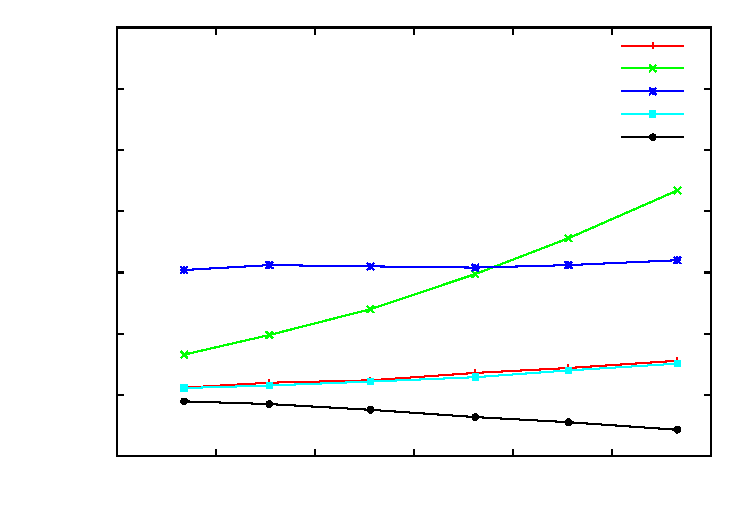
\includegraphics{head-losses-qa}}%
    \gplfronttext
  \end{picture}%
\endgroup

\caption{The various head losses versus $Q_A$.}
\label{fig:head-losses-qa}
\end{figure}
Values of the head losses across the various flow meters are given in
figure~\ref{fig:head-losses-qa}.

For the venturimeter, the head losses increase slightly with
an increase in $Q_A$. The corelation appears to be fairly linear.

For the orifice plate meter, the head losses increase significantly with
an increase in $Q_A$. The rate of this increase is in turn greater
at higer values of $Q_A$. Thus, there appears to be a higher order corelation.

For the rotameter, the head losses are fairly stable at all values of $Q_A$.
There appears to be no significant corelation.

For the wide-angled diffuser, the head losses increase slightly with
an increase in $Q_A$. The corelation appears to be fairly linear.

For the right-angled bend, the head losses decrease slightly with
an increase in $Q_A$. The corelation appears to be fairly linear.

\subsection{Proportionality between $Q$ and position of rotameter float}
The discharge through the rotameter float,
\begin{equation}
\label{eq:rotameter-discharge}
Q = 2\pi R_f L \theta v,
\end{equation}
\begin{tabular}{rll}
where &$R_f$& is the float radius, \\
      &$L$& is the height from the datum to the top of the float, \\
      &$\theta$& is the semi-angle of the tube taper, and \\
      &$v$& is the mean velocity. \\
\end{tabular}

$R_f$ is a property of the float and is thus constant. 
$\theta$ is a property of the rotameter tube and is thus constant.
Now, the weight of the float in water is balanced by 
the force due to the water moving at a certain velocity $v$.
The float will rise to the level at which this value of $v$ is attained.
This leaves $L$ as the only independent variable in 
equation~\eqref{eq:rotameter-discharge}. 
Thus, $Q$ is proportional to $L$.

\section{Conclusion}
The coefficient of discharge, $C_d$ was determined to be 
0.981 for the venturimeter and 0.601 fo the orifice plate meter.
The linear regression line with a 90\% confidence interval worked
out to be $y = (1.014 \pm 0.021)x - (12.76 \pm 1.81)$ for the
venturimeter and $y = (0.6160 \pm 0.0053)x - (9.829 \pm 0.747)$ for the
orifice plate meter.

There appears to be a positive linear corelation between the head losses across
the venturimeter and across the wide-angled diffuser with 
actual discharge, $Q_A$.
There appears to be a negative linear corelation between the head losses across
the right-angled bend with $Q_A$.
There appears to be a positive higher order corelation between the head losses 
across the orifice plate meter with $Q_A$.
Lastly, there appears to be no significant corelation between the head losses 
across the rotameter with $Q_A$.

Further analyses over a larger range of discharge values can be performed 
to ascertain more general corelations between the head losses and $Q_A$.
\end{document}
